
\chapter{Data Exploration}
\section{Introduction}
\paragraph{}
A good starting point for the analysis is to make some data exploration of the data set. The first thing to be done is statistical analysis such as counting the number of text per class or counting the number of words per sentence. The second step consit of doing Latent Dirichlet Allocation\cite{blei2003latent} in order to make unsupervised clustering of the text and see if there is some kind of correlation between the clusters to which a text belongs and its labels. 

\section{Dataset statistics}
\subsection{Fake News Corpus}
\subsubsection{General Analysis}
\paragraph{} Because \textbf{Fake News Corpus} is the main dataset, the data exploration will start with this dataset. And the first thing is to count the number of items per class. Before starting the analysis, it is needed to cleanup the dataset. As it is originaly given in a large 30GB CSV file, the first step is to put everything in a database in order to be able to retreive only wanted peice of information. In order to do so, the file have been red line by line. It appears that some of the lines are baddly formated, preventing them to be red correctly, in this case they are dropped without being put in the database. Also, each line that is a duplicate of a line already red is also dropped. The second step in cleaning the set consist of some more duplicate removal. Indeed, dropping same lines remove only exact duplicate. It appears that some news does have the same content, with slight variation in the title, or a different author. In order to remove the duplicate, each text is hashed using SHA256 and those hash a compared, removing duplicates and keeping only one. 

\paragraph{} Because the dataset have been cleaned, numbers provided by the dataset creators and number computed after cleaning will be provided. We found the values given at \textbf{Table \ref{tab:explo:count1}}. It shows that the number of fake news is smaller by a small factors with respect to the number of reliable news, but given the total number of items it should not cause any problems. But it will still be taken into account later on. 

\begin{table}[h]
\centering
	\begin{tabular}{l|r|r}
  Type & Provided & Computed\\
  \hline
  Fake News & $928,083$ & $770,287$\\
  Satire & $146,080$ & $855,23$\\
  Extreme Bias & $1,300,444$ & $771,407$\\
  Conspiracy Theory & $905,981$ & $495,402$\\
  Junk Science & $144,939$ & $79,342$\\
  Hate News & $117,374$ & $65,264$\\
  Clickbait & $292,201$ & $176,403$\\
  Proceed With Caution & $319,830$ & $104,657$\\
  Political & $2,435,471$ & $972,283$\\
  Credible & $1,920,139$ & $1,811,644$\\
  \hline
\end{tabular}
  \caption{Number of texts per categories}
  \label{tab:explo:count1}
\end{table}

In addition to the numbers provided at \textbf{Table \ref{tab:explo:count1}}, there are also two more categories that are in the dataset but for which no description is provided: 
\begin{itemize}
  \item Unknwon: 231301
  \item Rumor: 376815
\end{itemize}

\paragraph{} To have a better view of the distribution of categories, an histogram is provided at \textbf{Figure \ref{fig:chap1:hist1}}.

\begin{figure*}[h]
	\centering
	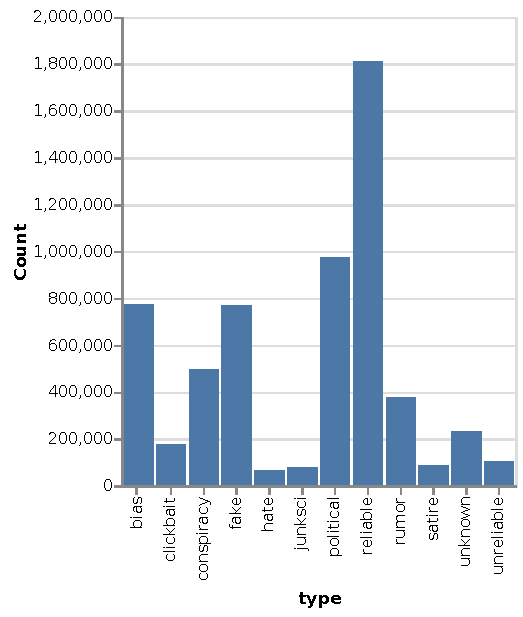
\includegraphics[width=0.5\textwidth]{chapter/images/data_exploration/plot1}
	\caption{Histogram of text distribution along their categories on the computed numbers. }
	\label{fig:chap1:hist1}
\end{figure*}

In addition, the number of words per text and the average number of words per sentences have been computed for each text categories. \textbf{Figure \ref{fig:data_explo:stats1}} shows the boxplots for these values. It can be seen that there is no significative difference that might be used in order to make class prediction. 

\begin{figure}[h]
  \centering
  \begin{subfigure}[b]{0.4\textwidth}
    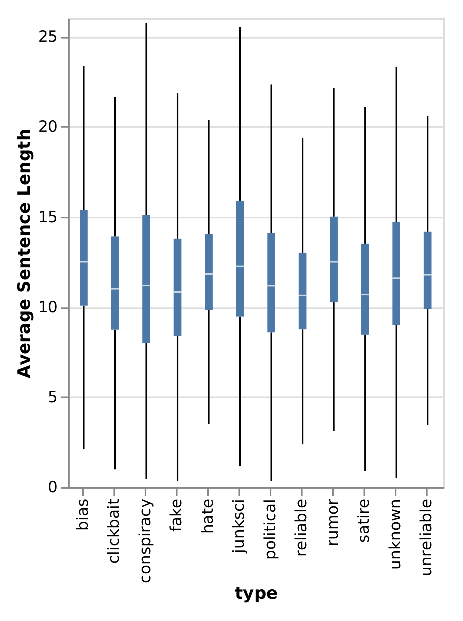
\includegraphics{chapter/images/data_exploration/boxplot_avgSentLen.eps}
    \caption{Boxplot of average sentence length for each category.}
  \end{subfigure}
  \hfill
  \begin{subfigure}[b]{0.4\textwidth}
    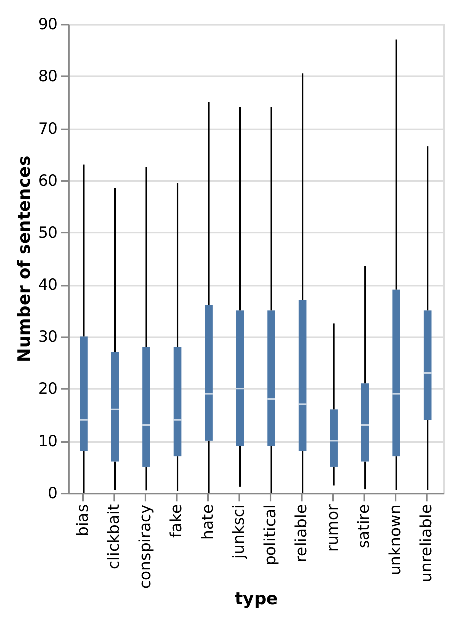
\includegraphics{chapter/images/data_exploration/boxplot_full_numSentences.eps}
    \caption{Boxplot of number of sentences for each category.}
  \end{subfigure}
  \caption{Summary statistics}
  \label{fig:data_explo:stats1}
\end{figure}

Before counting the number of words and sentences, the texts are preprocessed using gensim\cite{rehurek_lrec} and NLTK\cite{BirdKleinLoper09}. The first step consist of spliting text into an array of sentences on stop punctuation such as dots or questions mark, but not on commas. The second step consist on filttering words that are contained in these sentences, to do so, stopwords (words such as 'a', 'an', 'the'), punctuation, words or size less or equal to tree, non alpha-numeric words, numeric values and tags (such as html tags) are removed. Finnaly, the number of word still present is used. 

\begin{figure}[h]
     \centering
     \begin{subfigure}[b]{0.3\textwidth}
         \centering
         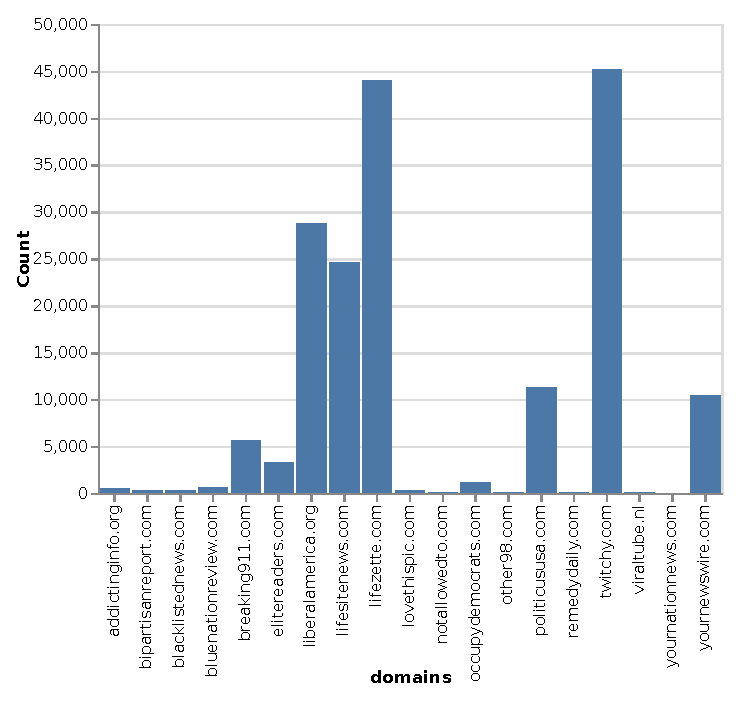
\includegraphics[width=\textwidth, height=0.3\textheight]{chapter/images/data_exploration/clickbait.eps}
         \caption{Clickbaits}
     \end{subfigure}
     \hfill
     \begin{subfigure}[b]{0.3\textwidth}
         \centering
         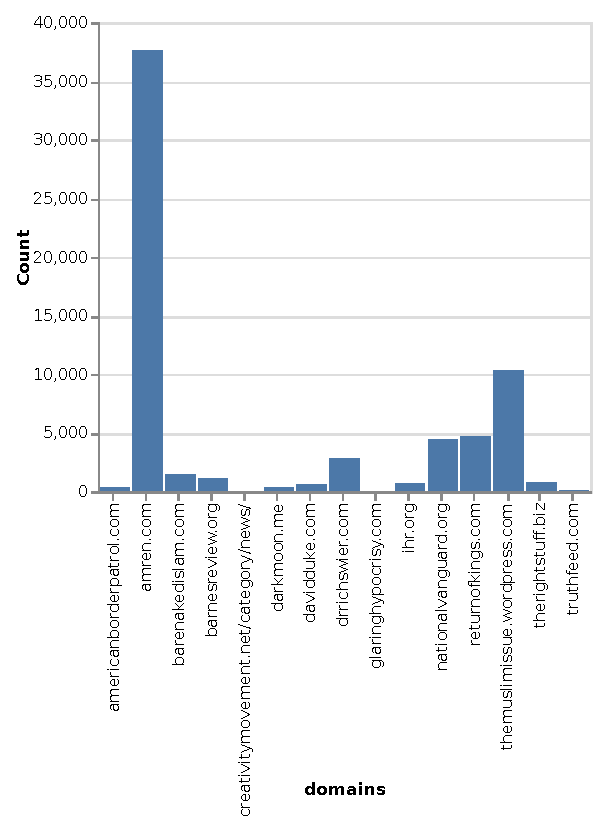
\includegraphics[width=\textwidth,height=0.3\textheight]{chapter/images/data_exploration/hate.eps}
         \caption{Hate}
     \end{subfigure}
     \hfill
     \begin{subfigure}[b]{0.3\textwidth}
         \centering
         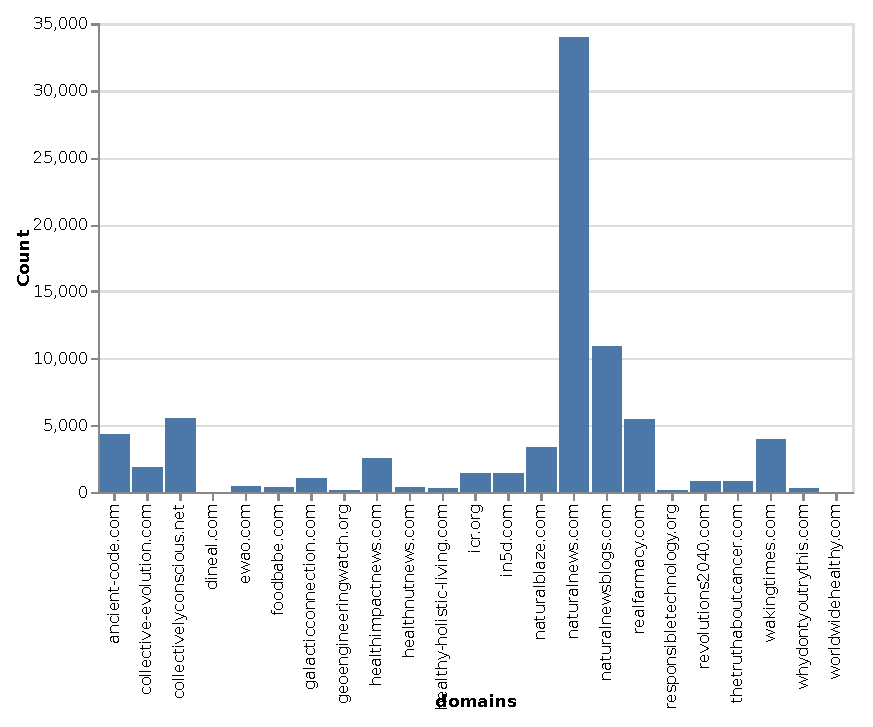
\includegraphics[width=\textwidth,height=0.3\textheight]{chapter/images/data_exploration/junksci.eps}
         \caption{Junk sience}
     \end{subfigure}
     \vfill
     \begin{subfigure}[b]{1\textwidth}
         \centering
         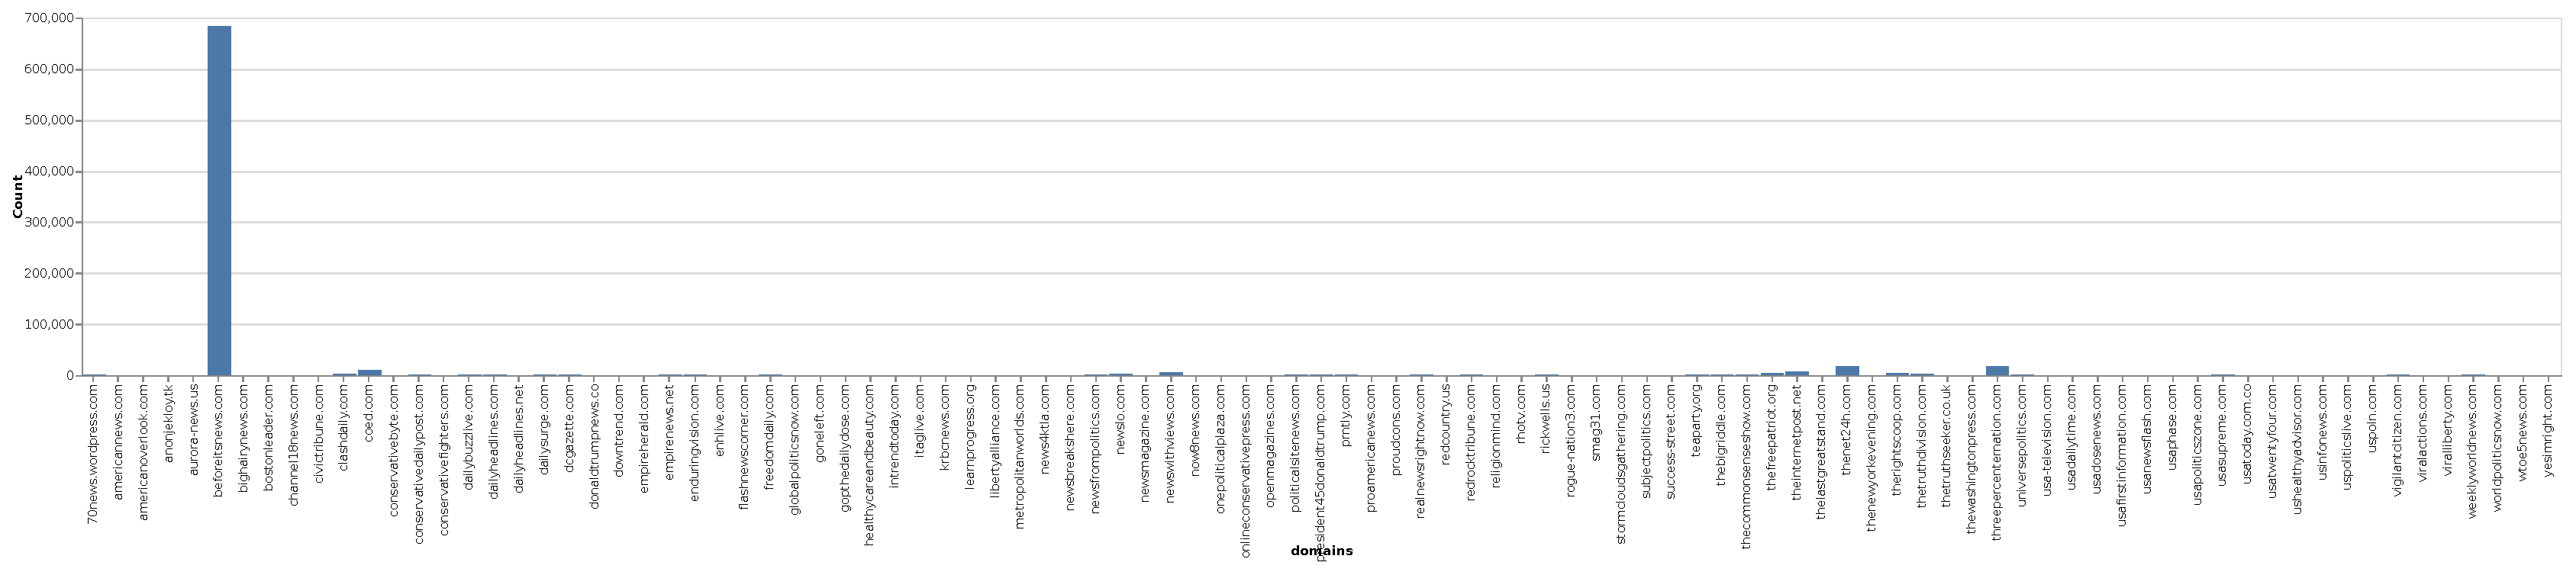
\includegraphics[width=\textwidth]{chapter/images/data_exploration/fake.eps}
         \caption{Fake}
     \end{subfigure}
     \vfill
     \begin{subfigure}[b]{1\textwidth}
         \centering
         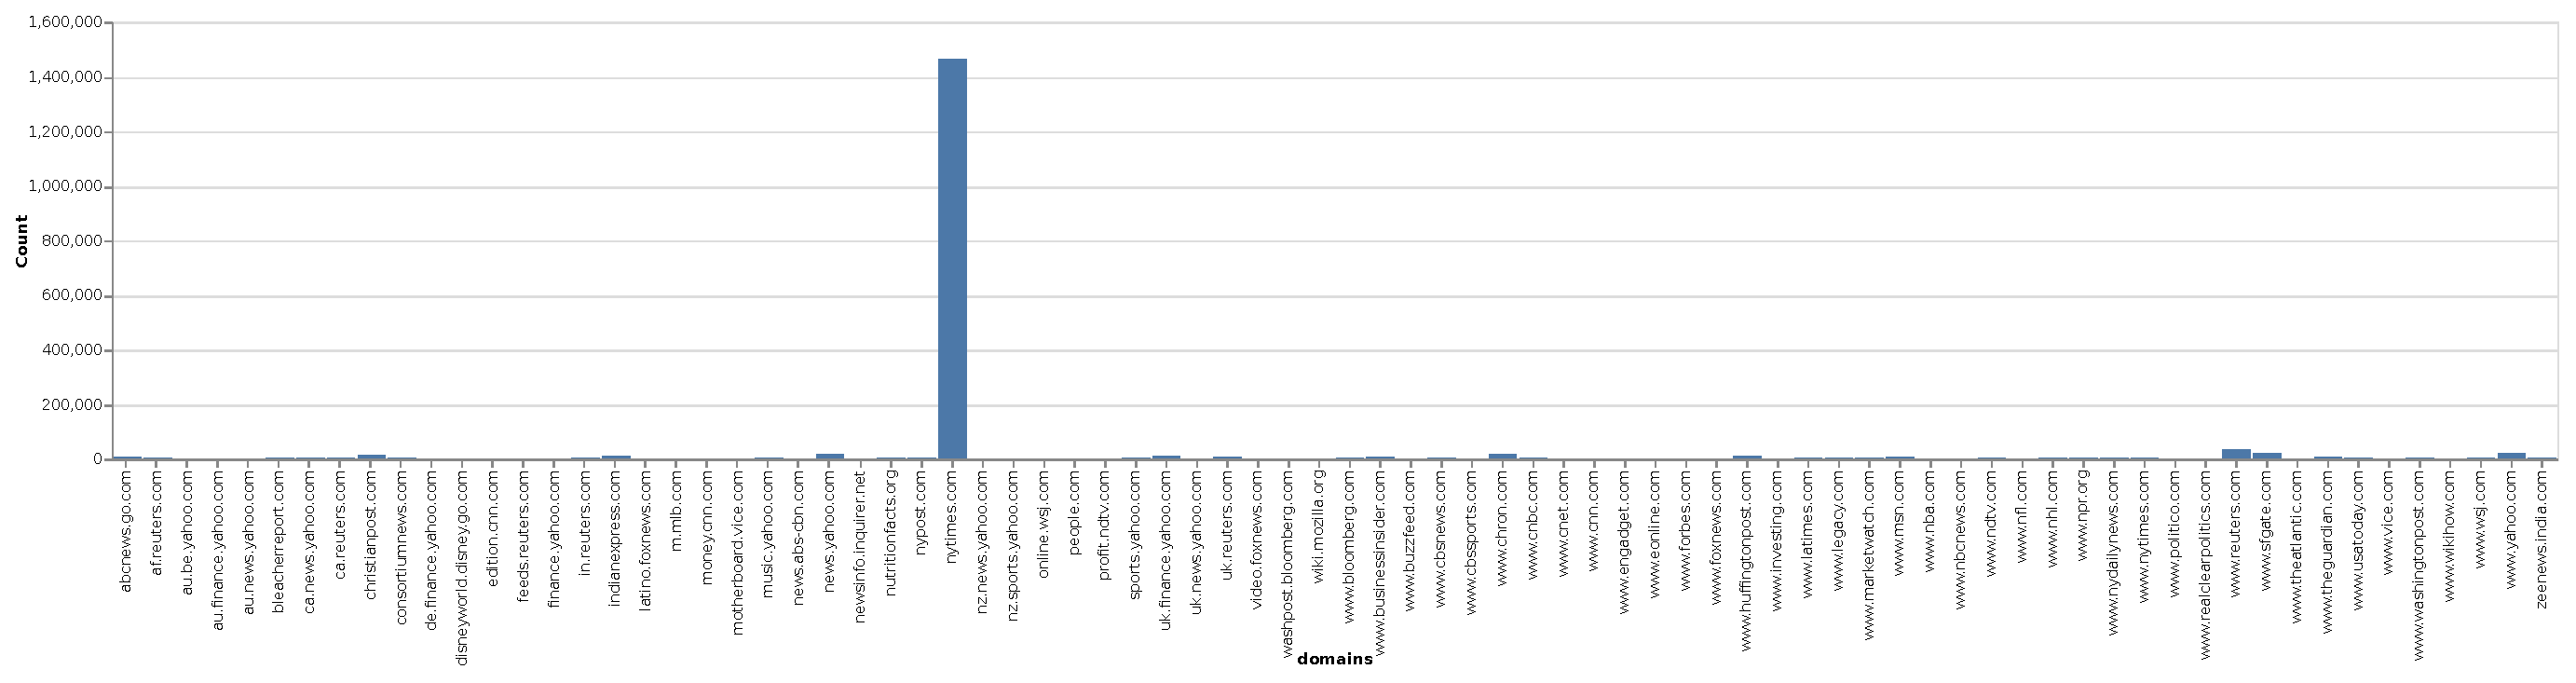
\includegraphics[width=\textwidth]{chapter/images/data_exploration/reliable.eps}
         \caption{Reliable}
     \end{subfigure}
\end{figure}
\begin{figure}\ContinuedFloat
    \begin{subfigure}[b]{1\textwidth}
         \centering
         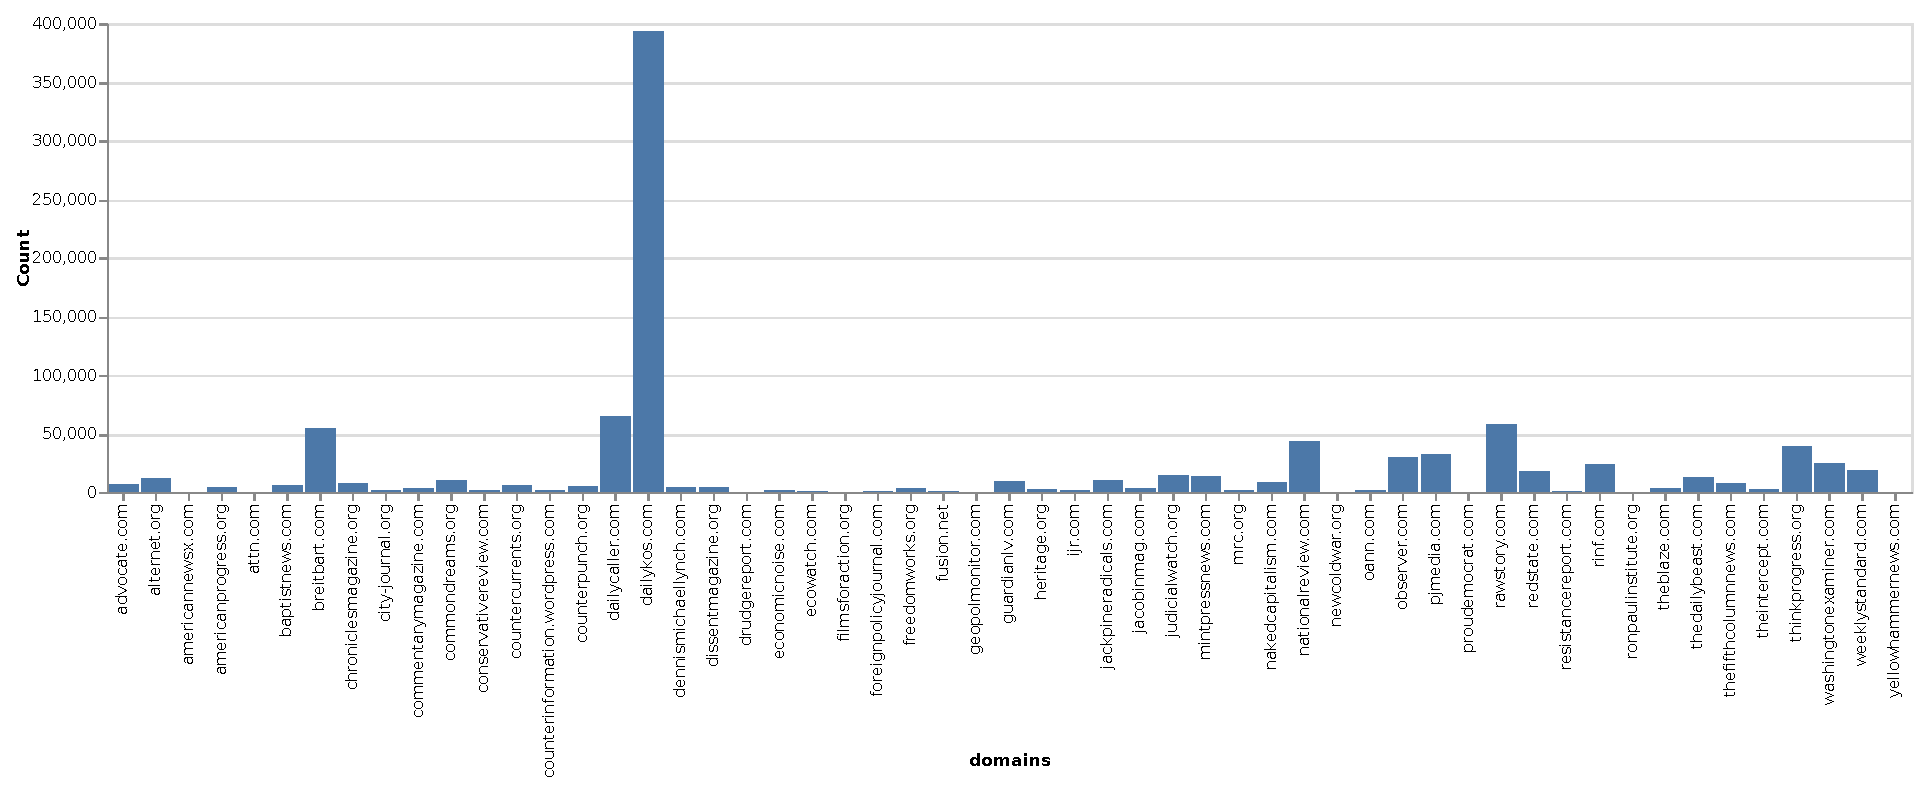
\includegraphics[width=\textwidth]{chapter/images/data_exploration/political.eps}
         \caption{Political}
     \end{subfigure}
     \vfill
     \begin{subfigure}[b]{1\textwidth}
         \centering
         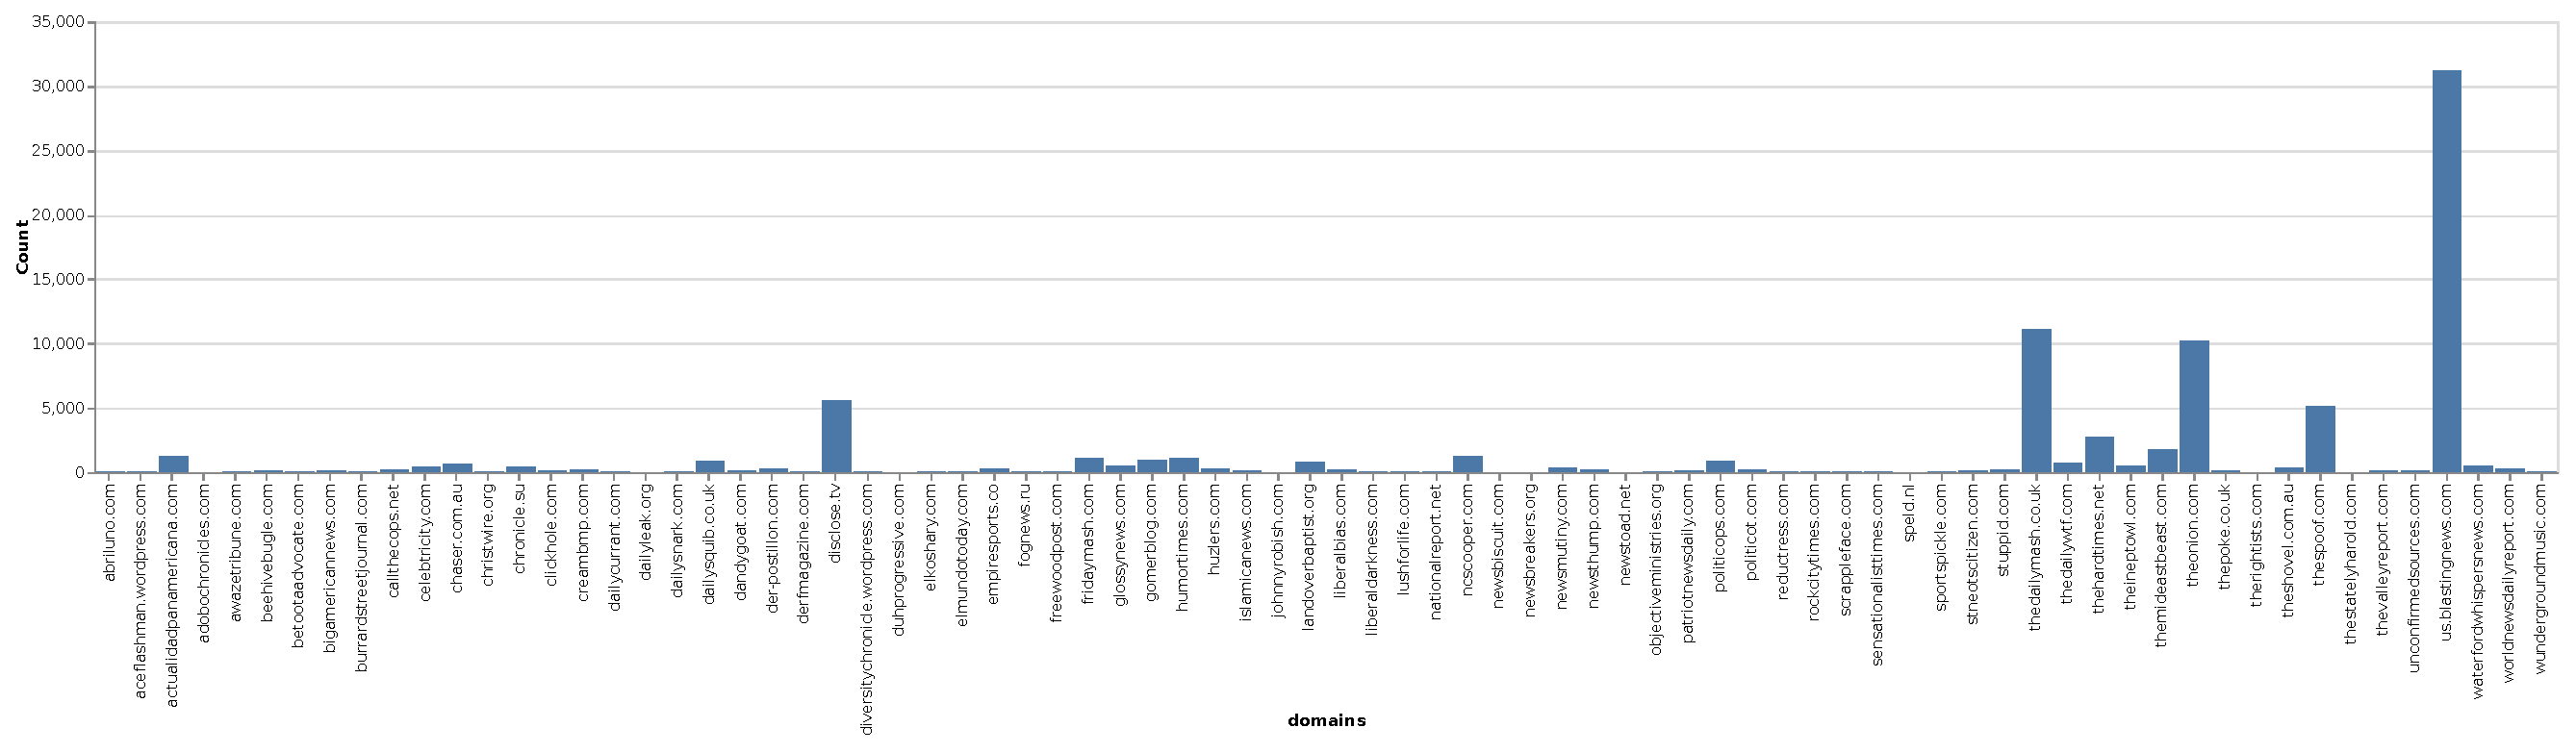
\includegraphics[width=\textwidth]{chapter/images/data_exploration/satire.eps}
         \caption{Satire}
     \end{subfigure}
     \vfill
     \begin{subfigure}[b]{1\textwidth}
         \centering
         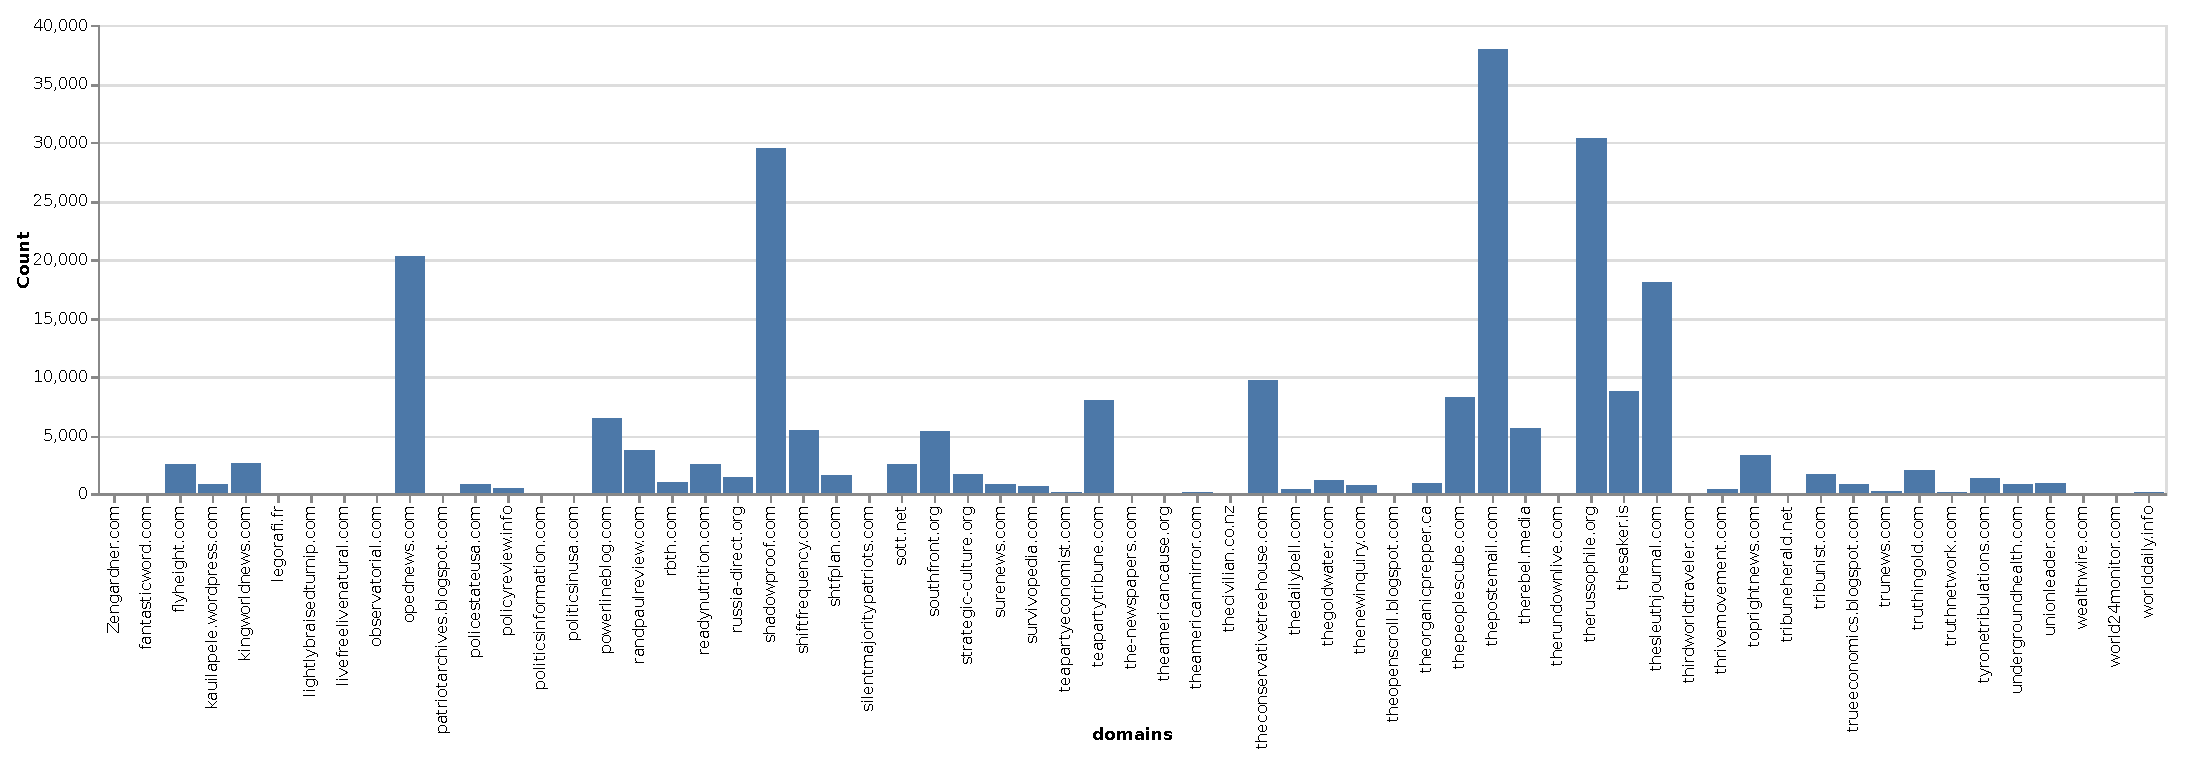
\includegraphics[width=\textwidth]{chapter/images/data_exploration/unknown.eps}
         \caption{Unknown}
     \end{subfigure}
        \caption{Histogram of news origin for each categories.}
        \label{fig:data_explo:source}
\end{figure}

\paragraph{} An interesting features to look at is the distrubtion of news sources with respect to their categories. It shows that in some case some source a predominant. For instance, looking at \textbf{Figure \ref{fig:data_explo:source}} shows that most of the reliable news are from \textit{nytimes.com} and in the same way, most of the fake news are comming from \textit{beforeitsnews.com}. That have to be taken into account when training and testing models as the goal is not to distinguish between these two sources but between fake news and reliable news. 

\subsubsection{Fake News analysis}
\paragraph{} In this section, the analysis will focus on fake news and reliable news. Because of what shows \textbf{Figure \ref{fig:data_explo:source}}, that is, some categories are almost all from the same source, an analysis of what happens when dropping these sources. First, lets compare the number of news while and while not taking into account majors sources. 

\begin{figure}[h]
  \centering
  \begin{subfigure}[b]{0.4\textwidth}
     \centering
     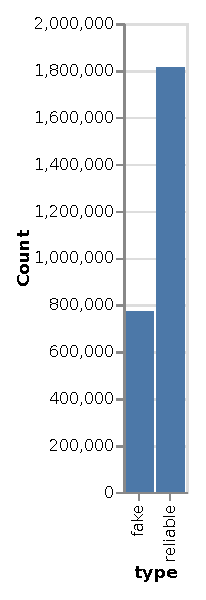
\includegraphics[]{chapter/images/data_exploration/notdown_hist.eps}
     \caption{}
     \label{fig:data_explo:hist2}
   \end{subfigure}
  \hfill
  \begin{subfigure}[b]{0.4\textwidth}
     \centering
     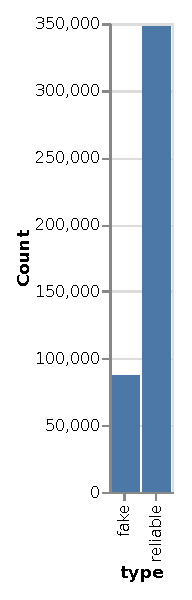
\includegraphics[]{chapter/images/data_exploration/downsampled_news_count.eps}
     \caption{}
    \label{fig:data_explo:hist3}
   \end{subfigure}
   \caption{\ref{fig:data_explo:hist2} is the number of news taking unto account \textit{nytimes.com} and \textit{beforeitsnews} and \ref{fig:data_explo:hist3} does not take them into account.}
\end{figure}

While removing these two sources, it still leaves enought texts to train the different models without the risk of learning somthing unwanted such as only separating these two sources. 

\begin{figure}
  \centering
  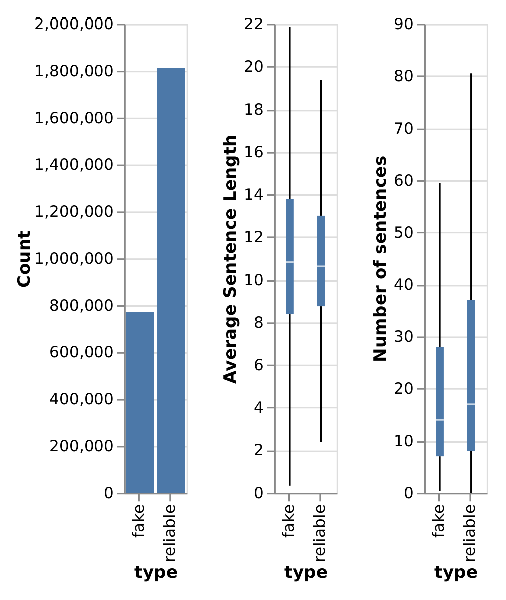
\includegraphics[]{chapter/images/data_exploration/not_downsampled.eps}
  \caption{Summary statistics for not downsampled fake and reliable news.}
\end{figure}